\documentclass[letterpaper, 11pt]{article}


%=================================================

\usepackage{fullpage, parskip}
\usepackage{fancyhdr}
\usepackage{amsmath, mathtools}
\usepackage{amssymb}
\usepackage[round,authoryear]{natbib}
\usepackage[breaklinks,backref,bookmarks=true]{hyperref}
\usepackage{varioref}
\usepackage{enumitem}
\usepackage{url}
\usepackage{graphicx}
\usepackage{tabularx}
\usepackage{subcaption}
\captionsetup{compatibility=false}
\usepackage[usenames,dvipsnames]{color}
\usepackage{pdfpages}
\usepackage{comment}
\usepackage{xspace}
%% Journal control sequences
\usepackage{aas_macros} 

%--------------------------------------------------
%% Header and Footer
\pagestyle{fancy}
\fancyhead{}
\renewcommand{\headrulewidth}{0.0pt}
\rfoot{Cato Sandford}
\lfoot{Summer 2012}

%%--------------------------------------------------
%% Maths macros
\def\psfobs{\ensuremath{{\rm PSF_{obs}}}\xspace}
\def\psfref{\ensuremath{{\rm PSF_{ref}}}\xspace}

\def\HST{HST\xspace}
\def\sextractor{SExtractor\xspace}
\def\psfex{PSFEx\xspace}
%%--------------------------------------------------
%% Language macros
\def\etc{{\&c.}\xspace}
\def\th{\textsuperscript{th}\xspace}
\def\ra{\ensuremath{\rightarrow}\xspace}
%%--------------------------------------------------
%% Editing macros
\def\TODO#1{ {\color{black}{\bf TODO: {#1}}}\xspace}
\def\MORE{{\color{red}{\bf MORE}}\xspace}
\def\REF{{\color{OliveGreen}{\bf REF}}\xspace}
\def\FIG#1{{\bf FIGURE: }{#1}}
%%=================================================


%% Top matter
\title{Discovery Sensitivity in Human Viewable Images}
\author{Cato Sandford\thanks{Department of Physics, New York University, USA; \texttt{cato@nyu.edu}}\\ \small with Phil Marshall and David Hogg}
\date{\today}

%%-------------------------------------------------

\begin{document}

\maketitle
\vspace{1cm}


\begin{abstract}
There is much scope in the future for ``crowd-sourcing'' the analysis of astronomical images. But the images will have to be presented in an intuitive and clear way so that non-experts have a shot at making an informed and useful contribution. In a summer project guided by David Hogg and Phil Marshall, I attempted to satisfy this need by devising a pipeline for the production of deconvolved RGB images from photometric telescope data.
\end{abstract}


\begin{center}
\line(1,0){250}
\end{center}
\vspace{-0.5cm}
\tableofcontents
\vspace{-0.1cm}
\begin{center}
\line(1,0){250}
\end{center}
\newpage


%%=================================================
%% Introduction
%%=================================================

\section{Introduction}
\label{sec:intro}

For centuries, astronomers have continued to astonish the world with pictures of a Universe far richer and more magnificent than any ordinary mind could conceive. Perhaps more than any other field of science, astronomy relies on the analysis of images to draw conclusions about the natural world. Indeed, new and unusual astronomical objects, such as
galaxies, nebulae, star clusters, supernovae and so on, appear readily to
experienced viewers as they inspect new images \citep[a recent example is the amateur discovery of a quadruple star system, reported in][]{PH12}; our understanding of  the structure of, for example, galaxies can
be improved by studying their morphology, by eye\footnote{Indeed, there is sometimes little alternative if one wants to draw meaningful conclusions about galaxy structure. It is beyond the scope here, but a discussion of what tasks can be effectively performed by computers and what cannot would be both very interesing and a compelling motivation for this work.} \citep[e.g.][]{Lah95, Lah++95, For++11, But11}\footnote{These references are selected to provide evidence of \emph{visual} inspection being useful.}.
Image viewing is a form of data exploration, an important step before making
quantitative measurements. But both exploration and measurement involve data
modeling, or inference: the viewer interprets the image in the context of a
model for that image that they hold.  By investigating and modeling this
viewing process, we can hope to increase the efficiency of such discoveries,
increasing the rate at which true detections are made, and reducing the
incidence of false detections. 

One way to increase the frequency with which discoveries are made  could be to
employ a larger number of experienced image viewers to look at images.  This
approach is being taken by ``citizen science'' projects such as Galaxy Zoo
(citation required). In the Galaxy Zoo system, color composite
images of galaxies are presented to large numbers of viewers, who carry out
visual morphological studies guided by a short questionnaire. The viewers have
a wide range of experience with astronomical images, and the majority of
viewers come to the site not having viewed many astronomical images before.
The model for astrophysical objects that this group has is therefore
data-driven: their ability to spot something new depends partly on their
pre-conceived notions of what galaxies look like, but to a greater extent it
will depend on the images they have seen in the system before. Given an
inspection Zoo and a user base like this,  how should we prepare and present
the color images of galaxies, to increase the probability of an interesting
new feature being detected? This is the question we seek to answer in this
paper, taking as our archetypal interesting features the faint arcs caused by
gravitational lensing. 

Gravitational lenses enable a wide range of science projects, providing a
means to measure the mass distributions of  galaxies, groups and clusters,
independent of their luminosity or dynamical state, and giving us a rare
magnified view of the distant universe. At present almost all these projects
are limited by the small samples of lenses known, but the wide field surveys
coming online have the potential to change that. A number of optical and near
infra-red imaging surveys are planned for the next decade that together have
been predicted to contain over 10,000 new gravitational lenses, an increase in
sample size relative to the present day of around two orders of magnitude
(see, for example, \citet{O+M10}; \citet{Paw++12}\footnote{The lensing discoveries of \citet{Paw++12} arose from the dedicated visual inspection of \HST images by two astronomers. They note that for the next generation of telescope missions, the time-demands of their method will be (even more) impractical. But their work lends credence to the claim that visual inspection may yet make valuable contributions to source-discovery.}; \citet[chapter 12]{LSST09}; \citet[chapter 1, page 8]{ERB10}). Most of these
surveys will be carried out on ground-based telescopes, and will be both
multi-filter, in many cases multi-epoch, and synoptic, in order to meet a wide
range of different science requirements. The thousands of square degrees of
sky imaged, and the billions of objects catalogued, will provide a huge mine
of data to be searched for rare objects like lenses. We expect image viewing
to play a role in this search process, most likely in the form of quality
control inspection of the outputs of various automated detection algorithms.

For an image to enable discovery, it needs to be {\it informative}: that is,
it must have high quality, so that interesting features are visible to the
viewer, and it must not be confusing, so that interesting features are not
mistaken for artefacts and ignored. The quality of an astronomical image is
only partly determined by the observing conditions, telescope, and camera: the
image processing carried out in software is also important. We have additional
information about the image that we can use to improve both its resolution and
depth. The stars provide images of the imaging system point spread function
(PSF), while our understanding of the detector and the sky background provide
a model for the noise in the image: we can attempt to use both of these in
reconstructing a higher quality image. There is a significant body of
literature on this image restoration process in astronomy \citep[e.g.][]{Ric72, N+N82, S+B84, P+P93, MCS98}. We might
expect algorithms like this to be important for synoptic surveys, whose
resolution and depth varies from image to image, and from filter to filter in
a partiular field of view. Combining raw images into a color composite will
produce colored artefacts due to the mis-matched resolution in the red, green
and blue channels; while the resulting composite will have different (mean)
resolution than other elsewhere on the sky, leading to an inhomogeneity that
will hinder the development of the viewers' internal feature model as they
have to allow for the variations in image quality. However, deconvolution is
notorious for producing image artefacts if not sufficiently regularized
\citep[see, for example, comments at the end of section~1 of][]{MCS98}: such artefacts could
create more problems than the deconvolution solves, reducing the probability
of a discovery being made.  An experimental test of the sensitivity with which
an image set enables discovery is required.

In this paper we investigate a simple model-based deconvolution scheme for
resolution matching, combined with a standardised image scaling and stretch,
producing homogenized sets of color composites for inspection and then testing
their sensitivity for lensed feature detection by viewers in the Galaxy Zoo.
Using a set of $N$ realistic simulated test images for the XXX survey 
containing faint lensed features, we define a set of metrics that quantify
discovery sensitivity based on a test group of viewers responses, and 
ask the following questions:

\begin{itemize}

	\item Does simple, ``light'' deconvolution designed for making
resolution-matched composite images introduce significant colored artefacts?

	\item What target PSF-width should be used in order to
maximise discovery sensitivity in the color composite images? How does this
relate to the input images' resolution?

	\item What algorithm for choosing the color composite images' stretch and
scaling should be used, to to maximise discovery sensitivity? 

	\item Is there significant scatter in viewers' preferences regarding image
stretching and scaling, such that viewer control over these parameters is
justified?

\end{itemize}

While we will focus on lensed features as our discovery targets, and the CFHT legacy
survey, we hope that our results will be of interest to the astronomical
community in general, and in particular to anyone who wants to see what they
have found in the object catalog database of a large synoptic imaging survey.

In the following two subsections, we discuss the origins of blurriness in telescope images (\ref{sec:psf}) and highlight some issues regarding the combination of band-pass data (\ref{sec:bands}). Then in section~\ref{sec:deconvolution} we outline a scheme for mitigating image bluriness. In section~\ref{sec:colour} we change tack and discuss a separate issue -- that of combining filtered images into coloured composites. These two strands are brought together in section~\ref{sec:combine}.


\subsection{The Point-Spread Function (PSF)}
\label{sec:psf}

An image of the sky taken with a telescope will never perfectly capture the information in the afferent light. One of the main problems is blurring -- precise points in the sky become fuzzy, extended objects when measured with any conceivable apparatus. This happens for two reasons: (i) the finite size of camera apertures or telescope mirrors spells trouble for geometrical optics; the resulting diffraction blurs the image formed at the detector. (ii) light wavefronts passing through the atmosphere to the surface of the Earth are inevitably distorted by density fluctuations, which affect the refractive index of the air. This is particularly tricky to correct for because the atmosphere changes in unpredictable ways, on short spatial and temporal scales. The problem can be circumvented to some extent -- a space telescope avoids corrupting its data with influence from the messy atmosphere. But putting a telescope in space is expensive and compromises the flexibility of the mission's science goals. Most of the time there is no alternative but to build a ground-based telescope and try to correct the blurriness.

We can talk about ``blurriness'' in a more quantitive way. An astronomical scene will typically feature a number of point sources (stars) which are bright but should be too small and distant to resolve into more than one pixel. How these point sources map to fuzzy blobs in our recorded image is known as the ``point spread function'' (hereafter PSF). As noted above, the PSF for a given image will have some contribution from the recording apparatus, and a more complicated time- and space-dependent contribution from the atmosphere.

So each pixel of the scene is replaced by a suitably weighted image of the PSF in the observed image: mathematically, this procedure is a convolution (see figure~\ref{fig:fuzz}).
In order to make precise inferences about the configuration or properties of astronomical objects, it is of utmost importance to find the PSF for a given image (or part of an image) and try to subtract it out as much as possible (``de-convolve'' in the astronomy jargon). A framework for estimating the PSF is given in section~\ref{sec:sextractor}, and the de-convolution process is described in the sections following.

\begin{figure}
	\centering
	\includegraphics[width=0.3\linewidth]{./Images/space2g}
	\includegraphics[width=0.3\linewidth]{./Images/space2conv}	
	\caption{The effect of the PSF: blurring and loss of distinctness.}
	\label{fig:fuzz}
\end{figure}


\subsection{Bandpasses and Colour Images}
\label{sec:bands}

As mentioned above, astronomical images are often filtered so that only a predetermined broad set of wavelengths will reach the detector. We then make multiple images of the same objects with different filters in place. This may seem strange: each filter throws away photons, making the resulting image less intense than an unfiltered counterpart. When we're trying to detect faint objects, this is not a good strategy. Furthermore, instead of taking just one picture of an object, we're now taking three or more (depending on the number of filters) -- this constitutes a considerable time burden on the telescope.

However, for many applications in the optical or near-optical, the sources of interest have ample brightness for us to use the filters. And the information we gain from having wavelength-dependent flux measurements is well worth the extra time required. With the colour-domain data, we can make all sorts of inferences about the age, activity, distance, chemical composition and temperature of an astronomical source. And these ``photometric'' images are much cheaper to collect (in terms of time and photon counts) than spectra of each individual object.

Once we have our three (say) images of the same patch of sky, with each representing a different colour, we may ask whether we can add them together recover a colour image as shown in figure~\ref{fig:coadd}. This seems reasonable, but in fact it can be very problematic. The three images have been made at different times; from section~\ref{sec:psf}, we know that they will have been corrupted by different PSFs; they may even have markedly different noise levels; indeed, atmospheric or device conditions may have resulted in spuriously different baseline intensities. As we can see from figure~\ref{fig:coadd_fuzz}, we have to do something cleverer than simply adding three such images to make a nice-looking colour composite. This will be discussed further in section~\ref{sec:colour}

\begin{figure}
	\centering
	\includegraphics[width=0.3\linewidth]{./Images/RGB_Channel_red}
	\includegraphics[width=0.3\linewidth]{./Images/RGB_Channel_green}
	\includegraphics[width=0.3\linewidth]{./Images/RGB_Channel_blue}\\
	\includegraphics[width=0.3\linewidth]{./Images/RGB_Channel_good_compos}
	\caption{Starting with three greyscale images (our R, G and B channels), we can create a colour composite image.}
	\label{fig:coadd}
	\vspace{1cm}
	\includegraphics[width=0.3\linewidth]{./Images/RGB_Channel_red}
	\includegraphics[width=0.3\linewidth]{./Images/RGB_Channel_green_conv5_noised}
	\includegraphics[width=0.3\linewidth]{./Images/RGB_Channel_blue}\\
	\includegraphics[width=0.3\linewidth]{./Images/RGB_Channel_red_compos}
	\caption{If the images to be combined are of differing quality (the green band now has more noise and larger PSF), adding them as we did before will result in an obviously distorted image. (Ignore the borders of the composite -- there is an image processing artefact there.)}
	\label{fig:coadd_fuzz}
\end{figure}


\subsection{The Data}

So the aim of the project is to start addressing these problems -- de-blurring images and combining them in such a way as to capitalise on their information content and emphasise faint features which may be of interest. I test my code on a sample of {\it irg} images from the CFHT Legacy Survey (CFHTLS). The hope is that the code will eventually be useful for large sets of images in the context described above.


\newpage
%%=================================================
%% DECONVOLUTION
%%=================================================
\section{Deconvolution}
\label{sec:deconvolution}

As mentioned in the introduction, it is frequently possible and indeed desirable to reduce or control the bluriness (or PSF) of a telescope image. In this section, we describe how one might do this -- the procedure is as follows:

\begin{enumerate}
	\item Identify the astronomical sources in a FITS image.
	\item Find the point sources, and from these estimate the PSF of the image. We call this the ``observed PSF'', or \psfobs.\label{pnt:getpsf}
	\item Generate a symmetrical\footnote{Well, not actually circularly symmetric.} target PSF for the image, using the dimensions and flux properties of the image PSF from point~\ref{pnt:getpsf}. We call this the ``reference PSF'' or \psfref.\label{pnt:PSF0}
	\item Create an object which maps the observed PSF to the reference PSF. This object is called the ``kernel'' and the mapping procedure is convolution.
	\item Apply this procedure to the original image; this should correlate all the pixels in such a way as to rid the image of asymmetrical blurriness and replace it with a blurriness of known properties.
	\item Finally, regularise the image by using some smoothing procedure.
\end{enumerate}

The reader may be confused at this point as to why, if we can correctly calculate the PSF of an image, we don't simply do away with the blurriness altogether -- i.e. find a kernel which maps the PSF to a point. This would be a ``hard deconvolution'', a procedure which is compellingly discouraged by the work of \cite{MCS98} (see appendix~\ref{sec:MCS98notes} for more discussion of this paper). Following this work, we may endeavour to obtain better knowledge of the sky by reducing the PSF, but we must avoid inadvertently violating the sampling theorem, which would certainly happen if we attempted a hard deconvolution.

Once we have made the target PSF as small as possible within this restriction, we can enforce that it be symmetrical uniform throughout the whole image: this is a ``soft deconvolution''. The result of this will be that all point sources have the same pre-determined shape, and extended sources will be superpositions of this shape.

Mathematically, we can think of \psfobs as being composed of the reference PSF convolved with a messy 2D function $K$:
\begin{align}
	\psfobs(\vec x) = \psfref(\vec x) \ast K(\vec x).
	\intertext{In the following sections, we discuss how we determine the observed PSF, construct the reference PSF, and find the convolution kernel $K$. Crucially for homogenising the image, we must also find the kernel $k$ which governs the inverse transformation, i.e.}
	\psfobs(\vec x) \ast k(\vec x) = \psfref(\vec x).
\end{align}

%%=================================================
%% SExtractor
%%=================================================
\subsection{Source Identification}
\label{sec:sextractor}

According to the list in section~\ref{sec:deconvolution}, the first step in deconvolving an image is to pinpoint and characterise all the sources in it. We do this using the \sextractor (``source-extractor'') software written by E. Beritn and hosted on the Astromatic website. \sextractor reads in a FITS image and catalogues all the astronomical sources it contains, for each one measuring useful parameters such as position, characteristics of shape and flux distributions. The identification of the distinct sources (``segmentation'') is based on a thresholding procedure, which compares regions of the image to the local background; this process is then repeated so that proximate objects can be deblended.\footnote{There is some discussion of replacing the threshold algorithm with wavelet decomposition in future editions of the software.} For more detail, see the user manual~\citep{sex96}, which can be downoaded from the Astromatic website~\url{astromatic.net}.

All the user really has to do is to decide how the program should be set up, and select -- from an impressive list -- which quantities should be calculated. I store the default settings in the config files  \texttt{prepsfex.sex} and \texttt{prepsex.param} respectively. The output of the program is a file with extension \texttt{.cat} (by default, if the image is called \texttt{image.fits}, the output will be \texttt{image.cat}). This contains information like the position, elongation and flux of the source, which is to be used by the next piece of software to estimate the PSF in the image.

%%=================================================
%% PSFEx
%%=================================================
\subsection{Determining the PSF of an Image}
\label{sec:psfex}

Another piece of Astromatic software, \psfex, is used here. From the FITS image and the information in the \sextractor's \texttt{.cat} file, \psfex identifies which objects are actually blurred point sources, and uses their shape to determine the image PSF. The selection criteria for finding the point soures is that they lie in a particular region on a plot of pixel-width versus object intensity. Inside this region, we can confidently say the oject is a star, while inside, the object could be a galaxy or a cosmic ray or noise or anything. More detail is given in the \psfex manual \citep{psfex11} -- see in particular figure~3 and section~6.2.1.

Again, there are a considerable number of options for how this estimation is done and what form the outputs take. After flirting with some of the more sophisticated options, it turns out that the key thing for my purpose is an integrated image of the average PSF for the image. For now at least, we're considering small images where the variation of the PSF over the field is small. We may have to do something rather more clever if we have to work with larger pictures in the future.


%%=================================================
%% PSF Generation
%%=================================================
\subsection{Generating a Target PSF}

We are now equipped with an image which estimates the PSF of our data, \psfobs. We now have to make a decision about what our reference PSF should look like.

In a (misguided) bid to keep things simple, I prescribed ``PSF-tidying'' rather than a traditional light deconvolution. This means that \psfref has the same size as \psfobs, but a different shape -- specifically, a 2D Gaussian. The procedure was:
\begin{enumerate}
	\item Find the centre and the two principal widths (variances) of the \psfobs image.
	\item Use this information to make a 2D Gaussian with the same position and widths.
	\item Save as a FITS file.
\end{enumerate}

Unfortunately, after many hours spent on making code compatible with this programme, a belated epiphany on the actual meaning of the Sampling Theorem meant that most of it had to be abandoned in favour of a much simpler procedure: viz., the target PSF should in all cases have a FWHM of two pixels.

My mistake was in applying the Sampling Theorem to the resolution of the data rather than the resolution of the detector. In retrospect, it's fairly obvious that this is wrong: the sampling increment should be twice as fine as the smallest feature in a signal. For an astonomical image, the sampling increment is a pixel and the smallest feature is the PSF -- so we should arrange it such that the PSF has a width of about two pixels.


%%=================================================
%% Kernel
%%=================================================
\subsection{Mapping from the Target PSF to the Observed PSF}
\label{sec:kernel}

In this section, we outline how to find the ``convolution kernel'' which maps between the two versions of the PSF, discussed above. This object allows us to regularise the entire image.

Say we have two similar images: $\mathcal{A}$, which is a picture taken by a real telescope; and $\mathcal{B}$, which represents the same astronomical image, with a smaller, user-specified PSF ($\psfref(\vec x)$). In order to change image $\mathcal B$ into image $\mathcal A$, we can convolve it by some kernel $k$:
\begin{equation}
	\mathcal A = \mathcal B \ast k.
\end{equation}
Note that $k$ is merely an image, or a template for how each pixel in $\mathcal A$ is a sum of pixels in $\mathcal B$.

Since convolution is a linear operation, we can cast our search for the convolution kernel in terms of a linear algebra problem. Specifically, we want to solve (for $\vec k$)\footnote{Here, and throughout the document, we abuse the vector/matrix notation. Vectors are traditionally defined by their transformation properties; here we just take them to be carfully-constructed lists of real numbers.} an equation of the form
\begin{equation}\label{eqn:vector}
	\vec a = \mathbf{B} \vec k,
\end{equation}
where the vector $\vec a$ and the matrix $\mathbf{B}$ encode the original and deconvolved image, and $\vec k$ represents the convolution kernel (also an image). When written in this form, our problem of finding $\vec k$ becomes a traditional vector-equation--solve.

The vectors $\vec a$ and $\vec k$ are easy to construct -- rows of the 2D image are concatenated into a long 1D array (this is called ``flattening''). If $\mathcal A$ is an image of $N$ pixels, then $\vec a$ will have $N$ elements. The kernel $\vec k$ has many fewer elements, but the procedure is exactly the same.

The target-PSF image matrix, $\mathbf B$ is less strightforward. We must think carefully about the convolution process to understand what's going on here. Consider a uniform $3\!\times\!3$ kernel being convolved with a $5\!\times\!5$ image, as shown in figure~\ref{fig:convolution_pix}. The form of the pixels suggests that it may be represented as the linear algebra operation shown in figure~\ref{fig:convolution_linalg}.

\begin{figure}
	\begin{center}\begin{tabular}{|c|c|c|c|c|}
		\hline
		1&2&3&4&5\\
		\hline
		6&7&8&9&10\\
		\hline
		11&12&13&14&15\\
		\hline
		16&17&18&19&20\\
		\hline
		21&22&23&24&25\\
		\hline
	\end{tabular}
	%
	\hspace{1mm} $\ast$ \hspace{1mm}
	%
	\begin{tabular}{|c|c|c|}
		\hline
		A&B&C\\
		\hline
		D&E&F\\
		\hline
		G&H&I\\
		\hline
	\end{tabular}
	%
	\hspace{1mm} = \hspace{1mm}
	%
	\begin{tabular}{|p{2.6cm}|c|c|}
		\hline
		1A+2B+3C+ +6D+7E+8F+ +11G+12H+13I & \ldots & \ldots\\
		\hline
		\ldots &\ldots &\ldots\\
		\hline
		\ldots &\ldots &\ldots\\
		\hline
	\end{tabular}\end{center}
	\caption{A five-by-five image (left) with pixels numbered from one to 25, is convolved with a three-by-three kernel (right) with pixels labelled from A to I. Notice the final image is smaller than the original -- more on this in section~\ref{sec:shave}.}
	\label{fig:convolution_pix}
\end{figure}

\begin{figure}
	\begin{center}
	$\begin{pmatrix}
		1&2&3&6&7&8&11&12&13\\
		2&3&4&7&8&9&12&13&14\\
		3&4&5&8&9&10&13&14&15\\
		&&&&\vdots
	\end{pmatrix}$
	%
	$\begin{pmatrix}
		A\\B\\C\\
		D\\E\\\vdots
	\end{pmatrix}$
	%
	\hspace{1mm} = \hspace{1mm}
	%
	$\begin{pmatrix}
		1A+2B+3C+\\+6D+7E+8F+\\+11G+12H+13I \\
		\vdots
	\end{pmatrix}$\end{center}
	\caption{The convolution procedure of figure~\ref{fig:convolution_pix} is translated into a matrix operation.}
	\label{fig:convolution_linalg}
\end{figure}


The $\mathbf B$ matrix of equation~\ref{eqn:vector} is then a matrix with ${\rm size}(a)$ rows and ${\rm size}(k)$ columns. Moreover, it has a skew-diagonal Toeplitz structure, which will help us to constuct it later.

Presently, the vector problem in equation~\ref{eqn:vector} is overdetermined (the kernel is smaller than \psfobs), so we must use some ``best fit'' procedure -- typically least-squares minimisation -- to find $\vec k$.

%%-------------------------------------------------------------------------------------------
\subsubsection{Pseudocode}

\texttt{\begin{enumerate}
	\item psf\_obs = readin(psfex\_psf.fits)
	\item psfmoments = moments(psf\_obs)
	\item psf\_ref = 2DGaussian(moments)
	\item \#\# Turn these image arrays into linear algebra objects
	\item psf\_obs = psf\_obs.flatten()
	\item psf\_ref = stack(psf\_ref, dim=(psf\_obs.size, kernel.size))\
 		\newline~\mbox{}~\hspace{1cm}\#\# stack() constructs rectangular matrix of dimensions dim\
 		\newline~\mbox{}~\hspace{1cm}\#\# conformable for multiplication with the flattened kernel image.
	\item kernel = solve(psf\_ref, psf\_obs)
	\item kernel = reshape(kernel, kernel\_dim)
	\item save\_image(kernel)
	\item return kernel
\end{enumerate}}

%%-------------------------------------------------------------------------------------------
\subsubsection{Interlude: Honesty Note}
\label{sec:shave}

When we convolve two images, we produce a new image pixel by taking a weighted sum of the surrounding pixels. For instance, say we convolve a large image $\mathcal{B}$ with a 3$\times$3-pixel image to get $\mathcal{A}$. The first (i.e. top-left) pixel of $\mathcal{A}$ that we can properly determine is not the same as the first pixel of $\mathcal{B}$, because we require input from the eight pixels around every $\mathcal B$ pixel in order to get an $\mathcal{A}$ pixel.

Thus, the honest thing to do is to throw away some information by making image $\mathcal A$ smaller than $\mathcal B$ -- in this example with a 3$\times$3 image, we shave off the four outer edges, so if $\mathcal B$ is $N\times M$, $\mathcal A$ is $(N-2)\times(M-2)$. A bigger convolving image would require more pixels to be lost from the result.

This contrasts with the traditional solution to the problem, which is to ``pad'' the original image with zeroes (see figure~\ref{fig:zeropad}) such that the final image is the same size as the (pre-padded) original was. This seems to introduce spurious information -- how can we possibly know that there are zeros at the border of an image? Often this is patently not the case, even for astronomical images which can be mostly black. With this in mind, it may seem preferable to adopt the ``lossy'' procedure outlined in the last paragraph.

DWH has argued semi-convincingly that we needn't make such a sacrifice in practice, because there is enough information in the border pixels to mitigate grave data-fabrication. See also the sections below, where this issue is discussed further in the context of a well-posed linear algebra problem.

\begin{figure}[h]
	\centering
	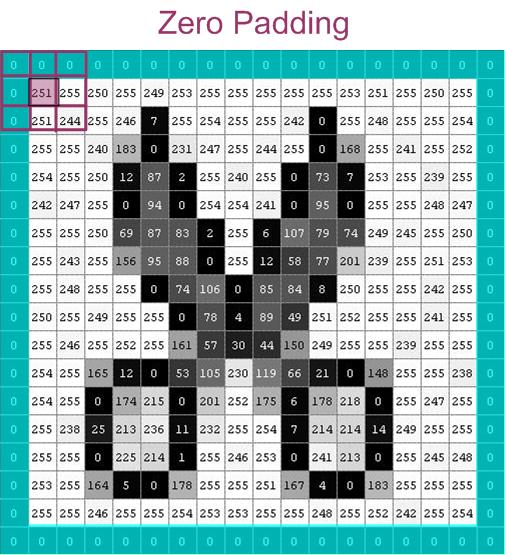
\includegraphics[width=0.33\linewidth]{Images/pad_zero_color.jpg}
	\caption{An image padded with zeroes. Convolution with the 3$\times$3 stencil will now preserve image size; but at what cost?}
	\label{fig:zeropad}
\end{figure}



%%=================================================
%% Deconvolution
%%=================================================
\subsection{Full Image Deconvolution}
\label{sec:imdec}

In section~\ref{sec:kernel} we found the kernel $k$ which would transform a PSF with known properties (\psfref) into the observed PSF (\psfobs). This same kernel can be used to transform an entire image with the observed PSF, $\mathcal A$, into the ``same'' image with the target PSF, $\mathcal B$. To do this, we can perform the operation
\begin{align}
	\mathcal{A} &= k \ast \mathcal{B},
	\shortintertext{or, in the language of linear algebra,}
	\vec{a} &= \mathbf{K} \vec{b}.\label{eqn:simple_deconvolve}
\end{align}
The image vectors $\vec a$ and $\vec b$ have the same form as discussed earlier -- they are simply flattened versions of the pixel-arrays. The kernel matrix $\mathbf K$ is more tricky; but after some refelxion, it transpires that $\mathbf K$ is a sparse, upper-diagonal matrix where every row is identical, but shifted right by one element with respect to the row above. (Note that in practice it is unweildy and prohibitively expensive to store all the zero-entries of the $\mathbf K$ matrix -- we have to be a little bit clever about how to store and manipulate the relevant information.)

Once we have constructed an appropriate kernel matrix, we solve (using \texttt{scipy.sparse.linalg}) the linear system to find the pixel vector $\vec b$ for the target image $\mathcal B$.

\paragraph{Solving an overconstrained problem.} If we want to solve the matrix equation~\ref{eqn:simple_deconvolve} and get an unambiguous answer, we need the system to be \emph{overdetermined} -- i.e. the inferred scene image-vector $\vec b$ should have fewer elements than the data image-vector $\vec a$. This goes right against the arguments raised in section~\ref{sec:shave}, which considers information-transduction in the convolution procedure.

How to resolve the conflict? Notice that in violating the section~\ref{sec:shave} mandate, we will introduce problems on the inferred image's boundaries\footnote{The problem will rach a full kernel-width into the recovered image, though the severity diminishes the further in you go.}. We can live with this -- especially if we are considering large images which have comparatively little information on the boundary. On the other hand, solving an underdetermined system is inherently unstable. So in order to arrive at a robust solution for $\vec b$, we should sacrifice our faithfullness to the convolution procedure.

Now there are two possibilities: (i) ``pad'' the data image $\mathcal A$ with zeroes; this will allow us to maintain the size of the inferred image. (ii) Keep $\mathcal A$ the same and accept a smaller inferred image $\mathcal B$. (In both cases, the kernel matrix $\mathbf K$ is taller than it is wide.) The choice isn't particularly compelling -- in (i) we are introducing spurious information but this is confined to the edges; in (ii) we maintain the purity of our method, but may introduce problems later on when we try to compare the images. Uncharacteristically, I'll opt for (i), the simpler-but-corrupt choice.

We should choose the padding so that the deconvolved image has the same size as the original data image. This means making a border of black pixels with total width ahnd height equal to the width and height of the kernel image. The changes to how we construct our kernel matrix are less trivial, and require careful thought and much picture-drawing (often it is hard to visualise how image manipulations translate into linear algebra operations). The kernel matrix corresponding to a 2D Gaussian kernel is shown in figure~\ref{fig:kernmat_pad}.

\begin{figure}[h]
	\centering
	\includegraphics[scale=1]{./Images/kernel.png}\\\vspace{1mm}
	\includegraphics[scale=1]{./Images/image.png}
	\includegraphics[scale=1]{./Images/image_pad.png}\\\vspace{1mm}
	\includegraphics[scale=0.1]{./Images/kernmat.png}
	\includegraphics[scale=0.1]{./images/kernmat_pad.png}
	\caption{Kernel matrix from the kernel image. Top: the convolution kernel. Middle row: the data (left) and the data padded all around with zeroes. Bottom: the matrix constructed from the kernel image in the case of the unpadded data (left) and the padded data (right).}
	\label{fig:kernmat_pad}
\end{figure}

The kernel matrix has some conspicuous gaps. For the unpadded case, this comed from the kernel overlapping the image boundaries. For the padded case, we also need to factor in the fact that there are many extra zeroes for which we must acconut. It should be clear from the shapes of the images in figure~\ref{fig:kernmat_pad} that the unpadded matrix is underconstrained and the padded matrix is overconstrained.

Note that all the black space in these matrices means we should be able to use sparse-matrix numerical packages to speed up computations.

%%-------------------------------------------------------------------------------------------
\subsubsection{Pseudocode}
\label{sec:decon_pseudocode}

This should illustrate how the general structure of the deconvolution procedure.
\texttt{\begin{enumerate}
	\item img\_array = readin(imagefile)\newline~\mbox{}~\hspace{1cm}\#\# Or can be given as straight array
	\item img\_vec = img\_array.flatten()
	\item krn\_array = readin(kernelfile)	\newline~\mbox{}~\hspace{1cm}\#\# Or can be given as straight array
	\item krn\_mat = sparse\_diag\_matrix(krn\_array.flatten(), offsets=[0,1,2,\ldots])\newline~\mbox{}~\hspace{1cm}\#\# general gist
	\item refimg\_vec = sparse\_lsq\_solve(krn\_mat, img\_vec)\label{pnt:sparse_solve}\
				\newline~\mbox{}~\hspace{1cm}\#\# System is underdetermined \ra iterative solution
	\item refimg\_vec = stretch(refimg\_vec)\newline~\mbox{}~\hspace{1cm}\#\# Ease of viewing
	\item refimg = reshape(refimg\_vec)\newline~\mbox{}~\hspace{1cm}\#\# Make into an image-worthy shape
	\item save\_image(refimg)
\end{enumerate}}

%%-------------------------------------------------------------------------------------------
\subsubsection{Incorporating an Initial Condition}

In practice, we can do better than this, since we have some prior information on what the deconvolved image should look like: viz. the original image. Using this guess could dramatically reduce the number of iterations required for convergence. This is how we do it.

We wish to solve an equation of the form
\begin{equation}
	\vec{a} = \mathbf{K}\vec{b}
\end{equation}
for $\vec b$. We have an initial guess, $\vec{b_0}$; from this we compute a residual vector,
\begin{equation}
	\vec{r_0} = \vec{a} - \mathbf{K}\vec{b_0}.
\end{equation}
If our initial guess is good, the elements of this vector should be small. Now we can find the correction to $\vec{b_0}$ by solving the matrix equation
\begin{equation}
	\mathbf{K}\vec{\Delta b} = \vec{r_0},
\end{equation}
using least-squares or something similar. Then our final estimate for the solution is
\begin{equation}
	\vec{b} = \vec{b_0} + \vec{\Delta b}.
\end{equation}
This should be more accurate and less computationally intensive than doing it without the initial condition.

For our purposes, the initial guess will just be the observed image; or in the language used above, $\vec{b_0}=\vec{a}$. However, we can't simply plough ahead with this, because the original image and the target image will have different dimensions ($\mathbf A$ is not square). This is easily rectified by augmenting the original image vector $\vec a$ with zeroes and using this padded version as $\vec{b_0}$; thankfully there is no ``dishonesty'' here (see section~\ref{sec:shave}), since $\vec{b_0}$ is only a guess in the first place.

We still have to be a little careful about how we achieve this padding: we shouldn't put zeros in the wrong places. If the original image was a square of side $n$ pixels, and the kernel image a square of side $m$ pixels, then the initial guess image should have side $n+m-1$ pixels. The vector $\vec{b_0}$ must therefore be padded with $(n+m-1)^2-n^2$ zeroes, distributed equally at the beginning and end of each stride. This could be achieved by doing the following:

\texttt{img\_vec\_padded = img\_vec.append(zeros(floor(m/2)), [[i*stride, -i*stride] }\\~\mbox{}\hspace{10cm}\texttt{for i in range(img\_vec.height)])},

or by embedding the original image into a larger array (this is what I actually do).

With all this in mind, it seems we modify our algorithm above:
\texttt{\begin{enumerate}
	\item img\_array = readin(imagefile)\
				\newline~\mbox{}~\hspace{1cm}\#\# Or can be given as straight array
	\item img\_vec = img\_array.flatten()
	\item krn\_array = readin(kernelfile)	\
				\newline~\mbox{}~\hspace{1cm}\#\# Or can be given as straight array
	\item krn\_mat = toeplitz\_matrix(krn\_array.flatten())
				\newline~\mbox{}~\hspace{1cm}\#\# general gist
	\item krn\_mat = sparse\_diag(krn\_mat)
	\item Dim = sparse\_lsq\_solve(krn\_mat, img\_vec - krn\_mat*img\_vec\_padded)\
				\newline~\mbox{}~\hspace{1cm}\#\# Find correction from residual
	\item refimg\_vec = img\_vec + Dim
	\item refimg\_vec = stretch(refimg\_vec)
				\newline~\mbox{}~\hspace{1cm}\#\# Ease of viewing
	\item refimg = reshape(refimg\_vec)
				\newline~\mbox{}~\hspace{1cm}\#\# Make into an image-worthy shape
	\item save\_image(refimg)
\end{enumerate}}

Having said all this, it is unclear how much benefit we actually get from including our prior information. The least-squares algorithm is convex, and has been well-optimised so it is also very fast\footnote{\texttt{linalg.lstsq} uses ``householder bidiagonalization'' to decompose matrices. For an $m$ by $n$ matrix, the complexity will be $\mathcal{O}(\max(m, n) * \min(m, n)^2$.}. Should test this, but it's not central to the project so maybe some other time.


%%-------------------------------------------------------------------------------------------
\subsubsection{Testing and Problems with Deconvolution Implementation}
\label{sec:decontest}

Now that the theory is in place, we can write a program which takes an image and deconvolves it to a constant PSF. But before we consider real astronomical images (e.g. from the CFHTLS catalogue we're using here), we should test the code in a situation where we know beforehand what to expect.

It is a remarkable property of Gaussian functions that that the convolution of two Gaussians is another Gaussian:
\begin{equation}
	\mathcal{G}(r,\sigma_1^2) \ast \mathcal{G}(r,\sigma_2^2) = \mathcal{G}(r, \sigma_1^2+\sigma_2^2).
\end{equation}
This suggests that a good test problem would be a Gaussian scene (of width $\sigma_1$) and a Gaussian kernel (width $\sigma_2$): the observed image will be a third Gaussian with the quadrature-sum width. Our code should be able to infer any one of the three objects from the other two.

The results of such a trial are given in figure~\vref{fig:hoggtest}. Simple code to illustrate exactly what I'm doing with this test is on page~\pageref{cde:hoggtest}.

\begin{figure}[h]
 	\def\width{0.2\linewidth}
 	\def\scale{2}
 	\centering
 	\includegraphics[scale=\scale]{"../test/hoggtest_data_true"}
 	\includegraphics[scale=\scale]{"../test/hoggtest_data"}\\ \vspace{1mm}
 	\includegraphics[scale=\scale]{"../test/hoggtest_scene_true"}
 	\includegraphics[scale=\scale]{"../test/hoggtest_scene"}\\ \vspace{1mm}
 	\includegraphics[scale=5.64\scale]{"../test/hoggtest_kernel_true"}
 	\includegraphics[scale=5.64\scale]{"../test/hoggtest_kernel"}
 	\caption{From top: data, scene and kernel images (scaled 2x,2x,6x) produced with the scheme outlined in section~\ref{sec:decontest}. On the left is the ``correct'' image (2D Gaussian). On the right is output of program: scene convolved with kernel; data deconvolved with that kernel; and the kernel inferred from the scene and the data.}
 	\label{fig:hoggtest}
\end{figure}

We can note immediately that there is some problem. Leaving aside the mess of the inferred scene for a moment, we can observe that the kernel is clearly not a Gaussian. This is strange, because the kernel calculation is a highly over-constrained linear algebra problem, so there should be no ambiguity from that end.

It gets worse. It turns out that the shape of the inferred kernel image (already wrong) is sensitive to the size we specify for the image. In figure~\ref{fig:inferred_kernel_sizes}, I show the kernel output by my \texttt{get\_kernel} routine for a variety of requested kernel image sizes (all else is equal).
\begin{figure}
	\centering
	\def\scale{2}
	\includegraphics[scale=\scale]{../test/hoggtest_kernel_9}
	\includegraphics[scale=\scale]{../test/hoggtest_kernel_11}
	\includegraphics[scale=\scale]{../test/hoggtest_kernel_13}	
	\includegraphics[scale=\scale]{../test/hoggtest_kernel_15}
	\caption{A variety of kernels inferred from a Gaussian data image and scene image. The difference between the images is only the dimesnsions of the image required for the output -- but obviously there is something else going on here too. The sizes are 9, 11, 13 and 15 pixels. They should all be 2D Gaussians of width three pixels.}
	\label{fig:inferred_kernel_sizes}
\end{figure}

The fact that neither the kernel inference nor the scene inference is working indicates that something is wrong with the way we construct linear algebra objects from the images (everything else has been tested extensively and shown to work). However, I've been over the construction of the matrices a number of times and haven't spotted any mistake; as of writing, I'm stumped.

{\it Unfortunately this severely limits my ability to proceed with the rest of the work. Until resolve the problem, much of the rest of this document will have act as a ``placeholder'': the framework into which I place results / demonstrations of the code's effectiveness. This will be indicated in each section affected by the problem.}

\begin{figure}
	\begin{verbatim}
	def decontest():
			
		t0 = time.time()
		
		## Define true scene, kernel, and data
			## Arguments are image size, width of Gaussian (x,y), centre (x,y), total flux
		scene_t  = DT.Gauss_2D(*[31, 4., 4., 15, 15, 1.])
		kernel_t = DT.Gauss_2D(*[11, 3., 3., 5, 5, 1.])
		data_t   = DT.Gauss_2D(*[31, 5., 5., 15, 15, 1.])
		imsave("hoggtest_scene_true.png", scene_t)
		imsave("hoggtest_kernel_true.png", kernel_t)
		imsave("hoggtest_data_true.png", data_t)
		
		## Calculate data: convolve the scene with the kernel
		data = scipy.signal.fftconvolve(scene_t, kernel_t, "same")
		imsave("hoggtest_data.png", data)
		
		## Infer kernel: data = scene * k --> kernel
		kernel = DT.get_kernel(scene_t, data_t, [11,11], False)
		imsave("hoggtest_kernel.png",kernel)
		
		## Infer scene: data = scene * k --> scene
		scene = DT.deconvolve_image(data_t, kernel_t, False)
		imsave("hoggtest_scene.png",scene)
		
		print "Total time:", round(time.time()-t0,3), "seconds."
		
		return
	\end{verbatim}
	\caption{Illustrative code for the three tests which must be passed in order to show the deconvolution procedure is functioning properly: retrieve data from scene and PSF kernel; extract kernel from scene and data images; infer scene from kernel and data. The last two tests are of actual practical importance in this project.}
	\label{cde:hoggtest}
\end{figure}

\paragraph{Next step: deconvolving a larger image.} Once the simple deconvolution step works, I'll apply the same procedure to a larger image with several objects of size \psfobs; e.g. figure~\ref{fig:tiled}. The result should be a similar array of objects with smaller width.
\begin{figure}
	\centering
	\includegraphics[scale=1]{"../test/imdec_obig"}
	\caption{Bigger image to deconvolve}
	\label{fig:tiled}
\end{figure}

\paragraph{Next step: speeding it up.} It may be possible to do the linalg-solve without computing the kernel matrix and performing numerous matrix products. The syntax is something like \texttt{solve(function, b)}, where \texttt{function} would be the operation I use to get the kernel matrix.


%%-------------------------------------------------------------------------------------------
\subsubsection{Deconvolved Examples}

[Note this section is a placeholder. Once the deconvolution code works I will flesh it out with images.]

Now that we've satisfied ourselves that the deconvolution code works properly, we apply it to some astronomical images from the CFHTLS catalogue. In all cases, a kernel 15 pixels across was used to deconvolve to a PSF width of 2 pixels.

\FIG{Original \ra deconvolved image}

\TODO{Comment on shape / noise properties of deconvolved images}

%%-------------------------------------------------------------------------------------------
\subsubsection{Shortcomings}

That still isn't the end of the story, as equation~\ref{eqn:simple_deconvolve} has some important shortcomings:

\begin{enumerate}
	\item In using our recorded image to recover a ``better'' one (which bears more resmblance to the scene), we have ignored the existence of \emph{noise} in the data. This problem will be addressed in section~\vref{sec:pixvar}.
	
	\item The procedure outlined in this section may not be well-determined, so the solution may be flexible. Typically, this will introduce artefacts into the image, which, given the goals outlined in the introduction, would be highly unwelcome.\newline The reference image we have obtained at this point must be ``regularised'', or smoothed according to some well-motivated principles. One can find a good discussion of these principles in \citet{MCS98}: this paper is outlined in appendix~\ref{sec:MCS98notes}. Some comments on their mathematical procedure can be found in appendix~\ref{sec:MCS98procedure}. \newline Though it would be entirely possible to implement this for the current project (indeed, we have already generated much of the necessary data), it may well be more effort than necessary. A more modest regularisation scheme will eventually be proposed in section~\ref{sec:regularisation}.
\end{enumerate}




%%=================================================
%% Image Noise
%%=================================================
\subsection{Pixel Variance and Noise}
\label{sec:pixvar}

Here we outline how one may address the existence of noise in our original image -- this has been hitherto ignored.

First, consider how the solution $\vec y$ to the matrix equation
\begin{equation}
	\mathbf M \vec y = \vec b \label{eqn:matrix_eqn}
\end{equation}
is found. Typically we strive to minimise the sum of the squared-residuals (call this $S$) of the solution: that is, find successive values of $\vec {y_i}$ such that
\begin{equation} \label{eqn:sum_residuals}
	S_i = (\mathbf M \vec{y_i} - \vec b)^{\rm T}(\mathbf M \vec{y_i} - \vec b) \ra 0,
\end{equation}
where $i$ labels the iteration number. Clearly, if we find a vector $\vec y$ which exactly solves equation~\ref{eqn:matrix_eqn}, the square-residuals will sum to zero (moreover this solution is unique). In practice, we choose some small number $\epsilon$ such that once $S_i \leq \epsilon$, we accept the corresponding solution $\vec {y_i}$.

Now if our data are noisy, or worse if there are correlations between data points, we must accomodate this into our residual-minimisation procedure.

Say we know or can calculate the variance of each pixel, $\sigma_j^2$, and the covariance between pixels, $\sigma_{jk}$ ($j$ and $k$ label the pixels).  We express this information as a covariance matrix $\mathbf{C}$:
\begin{equation}
	\mathbf{C} =
	\begin{pmatrix}
		\sigma_1^2	& \sigma_{12}	& \sigma_{13}	& \ldots	& \sigma_{1N}\\
		\sigma_{21}	& \sigma_2^2	& \sigma_{23}	& \ldots 	& \sigma_{2N}\\
		\vdots		& \vdots 		&  \vdots		& \ddots & \vdots \\
		\sigma_{N1}	& \sigma_{N2} 	& \sigma_{N2}	& \ldots	& \sigma_N^2
	\end{pmatrix}
\end{equation}
(note that $\mathbf{C}_{jk}=\mathbf{C}_{kj}$).

Including this information in the solution amounts to modifying the expression for the summed residuals, \ref{eqn:sum_residuals}, in the following way:
\begin{equation}\label{eqn:matrix_eqn_noise}
	S_i = (\mathbf M \vec{y_i} - \vec b)^{\rm T}\mathbf{C}^{-1}(\mathbf M \vec{y_i} - \vec b).
\end{equation}

A good trick for achieving this result without re-writing our minimisation code is to trivially modify equation~\ref{eqn:matrix_eqn}:
\begin{equation}
	\mathbf M \vec y = \vec b \quad\longrightarrow\quad \mathbf{C}^{-\frac{1}{2}}\mathbf{M} \vec y = \mathbf{C}^{-\frac{1}{2}}\vec b.
\end{equation}
It is easy to show, using the symmetry of $\mathbf{C}$, that using this matrix equation in~\ref{eqn:sum_residuals} yields equation~\ref{eqn:matrix_eqn_noise}.



%%-------------------------------------------------------------------------------------------
\subsubsection{Pseudocode}

We modify the procedure of section~\ref{sec:decon_pseudocode} to accomodate the covariance matrix (we only really modify part~\ref{pnt:sparse_solve}, but for completeness here is the whole thing):
\texttt{\begin{enumerate}
	\item img\_array = readin(imagefile)\newline~\mbox{}~\hspace{1cm}\#\# Or can be given as straight array
	\item img\_vec = img\_array.flatten()
	\item krn\_array = readin(kernelfile)	\newline~\mbox{}~\hspace{1cm}\#\# Or can be given as straight array
	\item krn\_mat = sparse\_diag\_matrix(krn\_array.flatten(), offsets=[0,1,2,\ldots])\newline~\mbox{}~\hspace{1cm}\#\# general gist
	\item Chalf = sqrt(inverse(covariance\_matrix( img\_array )))
	\item refimg\_vec = sparse\_lsq\_solve(Chalf * krn\_mat, Chalf * img\_vec)\
				\newline~\mbox{}~\hspace{1cm}\#\# System is underdetermined \ra iterative solution
	\item refimg\_vec = stretch(refimg\_vec)\newline~\mbox{}~\hspace{1cm}\#\# For ease of viewing
	\item refimg = reshape(refimg\_vec)\newline~\mbox{}~\hspace{1cm}\#\# Make into an image-worthy shape
	\item save\_image(refimg)
\end{enumerate}}


%%=================================================
\subsubsection{Noise Model}
\label{sec:covariance_matrix}

Having established that our minimisation functional, $S$, should include the data covariance matrix $\mathbf C$, we must now discuss how to calculate this matrix.

The most trivial thing to do is what we have done thus far: neglect all the noise in the data. This corresponds to taking
\begin{equation}
	\mathbf C = \mathbb{I},
\end{equation}
such that all $\mathbf C$s in the above equations disappear.

If we actually want to take the noise into consideration, the easiest thing to do would be to assume (i) that each pixel represents an independent measurement (i.e. $\mathbf{C}_{jk}\propto \delta_{jk}$: there are no off-diagonal elements); and (ii) that each pixel in the image has the same uncertainty $\sigma$ associated with it (this uncertainty $\sigma$ is simply the root-variance of all the pixel values). Thus,
\begin{equation}
	\mathbf C = \sigma^2\mathbb{I}.
\end{equation}

Increasing the sophisitcation of our model further, we could relax condition (ii) above and let different pixels have different noise levels\footnote{I believe one would describe this variable noise model as ``heteroscedastic''.}. This makes a lot of sense, since we'd expect brighter pixels to have higher noise. To get an idea of why this might be, consider photons from the sky arriving on a (perfect) telescope detector. This is a prototypical Poisson process, and in accordance with Poisson statistics, the mean count for a particular pixel will be equal to the variance in that pixel. In situations where there are many photons arriving at our detector (e.g. looking at bright optical sources), our Poisson distribution will become a Normal distribution; but the equality of mean and variance wil still hold. These considerations suggest the following covariance matrix:
\begin{equation}\label{eqn:covmat}
	\mathbf{C}_{jk} = \frac{n_j}{n}\sigma^2\delta_{jk},
\end{equation}
where $n_j$ is the number of counts in pixel $j$, $n$ is the total number of counts in the entire image. Note that this matrix is still diagonal, and the overall noise properties of the image are preserved.

This is a pretty rudimentary model for the pixel uncertainty. A more methodical / unprejudiced procedure might be to use ``feasible generalised least squares''. But that's the general gist.

Now consider condition (i) above: is it possible that the noise in pixel $j$ is correlated with the noise in pixel $k$? The answer is yes, for two reasons. First, a well-resolved source will be spread over several pixels. These pixels will have similar (high) noise levels when compared to the background, so neighbouring pixels have correlated noise. The second reason comes from considering the limitations of the detector. Take for example a CCD grid: very bright sources may saturate pixels if the exposure time is long. Charge, or photon counts, will overflow into neighbouring pixels, coupling the intensity and the noise.

A covariance matrix which refelcts these considerations will have off-diagonal elements which appear in diagonal stripes directly either side of the main diagonal (representing sideways-neighbours of pixel $j$) and other diagonal stripes around $w$ elements from the main diagonal, where $w$ is the width of the image. A calculation of how these off-diagonal stripes are related to the diagonal value $j$ will depend to some extent on the intensity profile of the source which appears in $j$ and on the properties of the detector. 

Still more advanced noise models will exist. But for our treatment, we will content ourselves with a covariance matrix of the form given in equation~\ref{eqn:covmat}.


%%-------------------------------------------------------------------------------------------
\subsubsection{Pseudocode}

This pseudocode illustrates how we compute the covariance matrix in equation~\ref{eqn:covmat}.
\texttt{\begin{enumerate}
	\item img\_array = readin(img\_file).flatten()
	\item flx\_tot = sum(img\_array)
	\item flx\_var = variance(img\_array)
	\item covmat = zero\_array( shape = [img\_array.size, img\_array.size] )
	\item covmat[i,i] = img\_array[i] for i in img\_array.size
	\item covmat *= ( flx\_var / flx\_tot )
\end{enumerate}}


%%-----------------------------------------------------------------------------------------
\subsubsection{Precomputed Covariance Matrices}

The necessity for locally calculating covariance matrices as in section~\ref{sec:covariance_matrix} is sometimes avoided if the data come packaged with precomputed covariance matrix. Rather than inferring the image properties solely from the image itself, it is preferable to trust the knowledge of the people who produced the data, who are more familiar with the properties (and possible malfunctioning) of the instrument. In the case of faulty or missing pixels, they can also provide ``masking arrays'' which block out the relevant pixels so they aren't involved in any inference downstream.


%%=================================================
%% Smoothing
%%=================================================
\subsection{Regularisation}
\label{sec:regularisation}

After deconvolution, there will sometimes be image artefacts, or ambiguity as to the ``best'' solution (e.g. in the case of an underdetermined problem). We can reduce these using a regularisation technique, which typically involves minimising a cost function associated with the distirbution of intensity in the image. Choosing the cost function will be to some extent a matter of preference, since it encodes many of our assumptions about what the image ought to look like.

\citet{MCS98} propose an effective regularisation scheme (see appendix~\ref{sec:MCS98notes}), but, as noted above, what they do may be overkill for our purposes. As of writing, this project hadn't reached the stage of incorporating a robust regularisation scheme; so this section is a placeholder for further work.


%%=================================================
%% Image Manipulation
%%=================================================
\subsection{Image Stretch}

A final comment about image viewability. The CFHTLS images with which we've been working have low photon counts, and the brightest sources often dominate to such an extent that other sources are invisible. To amend this, we've been applying a ``stretch'' to the image -- a re-scaling of intensities such that faint objects are made brighter without saturating bright pixels. Much of the work that went into the next section was concerned with how best to do this, but for now we just use a simple linear stretch:
\texttt{\begin{enumerate}
	\item a = median(img)
	\item b = precentile(0.975, img)
	\item sigma = 0.5*(b-a)
	\item scale\_min = a-5.0*sigma
	\item scale\_max = a+10.0*sigma
	\item img = (img-scale\_min)/(scale\_max-scale\_min)
	\item img.clip(scale\_max-scale\_min)
	\item save(img)
\end{enumerate}}
Figure~\ref{fig:linear_stretch} shows the results of the procedure performed on two images. Notice that the stretch also brightens the sky-level, and enhances noise.

\begin{figure}[h]
	\centering
	\includegraphics[width=0.3\linewidth]{../../Data/CFHTLS_03/CFHTLS_03_g_sci/CFHTLS_03_g_sci.png}	
	\includegraphics[width=0.3\linewidth]{../../Data/CFHTLS_03/CFHTLS_03_g_sci/Enhanced_Original/CFHTLS_03_g_sci_rescaled.png}\\\vspace{1mm}	
	\includegraphics[width=0.3\linewidth]{../../Data/CFHTLS_12/CFHTLS_12_i_sci/CFHTLS_12_i_sci.png}	
	\includegraphics[width=0.3\linewidth]{../../Data/CFHTLS_12/CFHTLS_12_i_sci/Enhanced_Original/CFHTLS_12_i_sci_rescaled.png}
	\caption{The effects of a simple linear stretch on the images CFHTLS\_03\_g.fits and CFHTLS\_12\_i.fits. Left is the raw data; the stretched version is on the right.}
	\label{fig:linear_stretch}
\end{figure}


\subsubsection{Noise Properties Post-Deconvolution}
\label{sec:deconvolution_noise}

We use stretches to make images more readily interpretable, and we will perform such procedures on original and deconvolved images alike. Since the overarching framework of this project is about pattern recognition, it is necessary to analyse the effects of such manipulations on the noise properties of the image. Below we show stretches of increasing severity on an original image and its deconvolved counterpart.

\TODO{Right column should be deconvolved image}

\begin{figure}
	\centering
	\def\width{0.15}
	\includegraphics[width=\width\linewidth]{../../Data/CFHTLS_06/CFHTLS_06_r/CFHTLS_06_r_sci}	
	\includegraphics[width=\width\linewidth]{../../Data/CFHTLS_06/CFHTLS_06_r/CFHTLS_06_r_sci}\\\vspace{1mm}
	\includegraphics[width=\width\linewidth]{../../Data/CFHTLS_06/CFHTLS_06_r/Enhanced_Original/CFHTLS_06_r_sci_rescaled2.png}
	\includegraphics[width=\width\linewidth]{../../Data/CFHTLS_06/CFHTLS_06_r/Enhanced_Original/CFHTLS_06_r_sci_rescaled2.png}\\\vspace{1mm}
	\includegraphics[width=\width\linewidth]{../../Data/CFHTLS_06/CFHTLS_06_r/Enhanced_Original/CFHTLS_06_r_sci_rescaled.png}
	\includegraphics[width=\width\linewidth]{../../Data/CFHTLS_06/CFHTLS_06_r/Enhanced_Original/CFHTLS_06_r_sci_rescaled.png}\\\vspace{1mm}
	\includegraphics[width=\width\linewidth]{../../Data/CFHTLS_06/CFHTLS_06_r/Enhanced_Original/CFHTLS_06_r_sci_rescaled02.png}
	\includegraphics[width=\width\linewidth]{../../Data/CFHTLS_06/CFHTLS_06_r/Enhanced_Original/CFHTLS_06_r_sci_rescaled02.png}\\\vspace{1mm}
	\includegraphics[width=\width\linewidth]{../../Data/CFHTLS_06/CFHTLS_06_r/Enhanced_Original/CFHTLS_06_r_sci_rescaled010.png}
	\includegraphics[width=\width\linewidth]{../../Data/CFHTLS_06/CFHTLS_06_r/Enhanced_Original/CFHTLS_06_r_sci_rescaled010.png}\\\vspace{1mm}
	\caption{The effects of a linear stretch on the appearance of the image CFHTLS\_06\_r. The stretch gets more severe as you go down, starting with the unstretched image. The image in the left column is the original data, while the right column is the deconvolved image.}
	\label{fig:deconvolution_noise}
\end{figure}



\newpage
%%=================================================
%% RGB
%%=================================================
\section{Bandpass Composition}
\label{sec:colour}

Telescope data is often given in ``bands'' -- we do not record the total flux coming from a point in the sky, but the flux in a certain wavelength range. This information allows us to investigate the properties of astronomical objects, such as temperature and chemical composition. However to make a readily-interprable image which contains maximum information in one hit, we need to combine the bands to make a colour-composite image. In all that follows, I use the mapping R=i, G=r, B=g.

Many methods had been developed to do this in accordance with researchers' individual aesthetic preference. But the full richness of possibility was still unexploited, until \citet{Lup++04} demonstrated just how much detail one could extract from data when colour was given its deserved treatment (see appendix~\ref{sec:Lup++04notes} for more detail). Using their method, we can combine images from different bands in a way which enhances hidden or faint features without allowing bright objects to dominate. It has the further advantage that the brightness of an object in the image is decoupled from its colour. The method is implemented in PJM's \emph{HumVI} (formerly \emph{ColorJPG}).

A further improvement to the method was implemented by Wherry. Whereas Lupton's algorithm is appropriate for tweaking the look of a single image to bring out interesting features, Wherry lets us standardise this manipulation across many images so their properties are comparable. We translated Wherry's improvements from IDL to Python, and integrated this module with the HumVI code. Some additional improvements are also made, such as increased versatility with rebinning.

%%-------------------------------------------------
\subsection{Comparison of Composition / Stretch Procedures}

The difference between the two procedures mentioned above (we'll call them ``lupton'' and ``wherry'') is subtle: the algorithms appear to be almost identical in how they combine and stretch the three input images. And though the methods appear to require different input parameters for the nonlinear stretch and colour scalings, this is deceptive.

Whereas lupton uses two explicit parameters, $Q$ and $\alpha$, to stretch an image ($\alpha$ is supposed to set the low-intensity scaling and $Q$ controls the saturation behaviour), wherry only takes one user-selected parameter to achieve this. However, this apparent distinction is spurious because the lupton parameters always appear together in the code as the product $\alpha Q$.

The other input is the list of three scalings, or weights, to be applied to the R, G and B channels of the image. Both methods give us control over these scalings -- a fact most important for our purpose, because we want to compare many composites against each other: a pixel of certain colour and intesnity in our final image should be representing the same raw data, regardless of the rest of the image.

The code for the lupton procedure (originally written by Patrik Jonsson) appears to be more versatile with the treatment of these scales. Default behaviour is for the code to choose the best scales for the image, by ensuring some threshold proportion of pixels which are saturated in each band. Or we can demand that the scale is the same for all three channels, so that the overall colour is preserved. Or we can select the scales manually and feed them into the program. This last behviour is the default (and only) for the current wherry implementation. It seems to me that this degree control is desirable, but we should defer conclusion until we see enough images: how much work is it for the user to select their own scales, and does the automatic selection of the lupton code produce ``natural''-looking images whose features are clear?

The most obvious distinction between the methods (rather than the implementation) is the inclusion in wherry of additional options on how to tweak the image: for example rebinning and modifying saturation levels. Beyond that, I can't tell. Maybe there's something subtle happening too.

\begin{figure}[h]
	\centering
	\includegraphics[width=0.4\linewidth]{{../examples/composed_lupton_10,0.04_Auto}.png}
	\includegraphics[width=0.4\linewidth]{{../examples/composed_10,0.04_Auto}.png}
	\caption{Comparing the results of combining the i, r and g bands of CFHTLS\_27\_sci using lupton (left) and wherry (right). The same nonlinearity parameters and colour scalings were used for both images.}
	\label{fig:lupton_wherry}
\end{figure}

Figure~\ref{fig:lupton_wherry}, we see that as expected the methods produce very similar results in terms of colouration and and intensity. However, the wherry image clearly has much higher noise levels, which sensibly degrade the image quality.

%%-------------------------------------------------
\subsection{Pseudocode for ``wherry'' Composition}

Here are the general steps in the code for a run of the wherry procedure.

\texttt{
\begin{enumerate}
	\item RGB = [readin(R\_data),readin(G\_data),readin(B\_data)]		\#\# *\_data can be filename, array of data, or a channel instance
	\item rescale(RGB, scalefactors)	\#\# multiply each band by a given number
	\item rebin(RGB, xrebinfactor,yrebinfactor)		\#\# re-sample images
	\item kill\_noise(RGB, cutoff)	\#\# sets all pixels below a threshold to 0
	\item arsinh\_stretch(RGB, nonlin)
	\begin{itemize}
		\item pixtot = R\_array+G\_array+B\_array	\#\# collapse images onto each other
		\item if pixtot[i,j]==0: pixtot[i,j]=1
		\item factor = arsinh(nonlin*pixtot)/(nonlin*pixtot)
		\item (R\_array,G\_array,B\_array) *= factor
	\end{itemize}
	\item if stauratetowhite is False: box\_scale(RGB)
	\begin{itemize}
		\item maxpixel[i,j] = max(R[i,j],G[i,j],B[i,j])	\#\# i.e. find the maximum pixel value of the three arrays
		\item if maxpixel[i,j] < 1: maxpixel[i,j]=1
		\item (R\_array,G\_array,B\_array) /= maxpixel
		\item (Also translates origin of image if required)
	\end{itemize}
	\item overlay/underlay \#\# not entirely sure what these are for
	\item scipy.misc.imsave(RGB)
\end{enumerate}}



\newpage
%%=================================================
%% UMBRELLA
%%=================================================
\section{Combined Deconvolution and Colour}
\label{sec:combine}

One of the first questions we asked was how to combine images of different qualities and still make the most of the information in each one; how do we prevent the low-quality images from poisoning the combination? For instance, say we have i-, r-, and g-band images of a galaxy, but by chance atmospheric fluctuations the r-band is very blurred. If we simply add the images together pixel by pixel, we'll end up in a situation like figure~\ref{fig:fuzz}, where the colours were distorted. Since colour is an important astronomical diagnostic, if this happens we'd be in trouble.

We now have the tools to begin solving this problem. Clearly we want to homogenise the blurriness of each of our R, G and B channels; that is make sure they have the same PSF. With these deconvolved raw imagess in hand, we can combine them \`a la section~\ref{sec:colour} to get a clean-looking result.

\TODO{Examples? Don't have good data to do this? Can't deconvolve yet?}


%%-------------------------------------------------
\subsection{Finding Optimal Parameters for Image Manipulation}

Recall that the overarching goal into which this project fits is to make certain features in astronomical imaged readily apprent to human veiwers. At some point, the free parameters of our procedure must be decided, in line with this aim; the best way to achieve this is to test the results of different stretches, scales and deconvolution properties on subjects who can rate the images on their clarity and the distinctness of fine structure.

PJM has this to say on the subject: `Anupreeta More has made a very nice set of test CFHTLS images for the
Lens Zoo, and I discussed with her a bit your work: she thinks we
should do a blind taste test at some point, showing the lens zoo dev
team her images that have been a) displayed in standard form with
HumVI and b) deconvolved and then
displayed in standard form with HumVI, and ask for them to be graded
for arc visibility. We can also do image testing at Adler Planetarium on the willing public there. The question we want to answer is: ``how should we display an image to maximize the likelihood of an untrained human seeing interesting feature X?'' '


%%-------------------------------------------------
\subsection{Quality Metrics}

But before troubling astonomers or members of the public with such requests, we should first try to rate the processed data with some objective measures of their quality. I haven't yet explored any of this to the extent of implementation, but here are a few ideas which might be a good starting point.
\begin{itemize}
	\item There will always be error in the minimisation step when we're solving the equation $\mathbf A \vec x = \vec b$. We can calculate the residual $\chi = \mathbf A \vec x - \vec b$, which will tell us how well our scene matches up with the data after convolution with the PSF kernel. The metric $\chi^2$ will provide an unambiguous indication of the ``goodness-of-fit'' of our model to the data.
	\begin{itemize}
		\item We take this further, by devising a protocol for splitting the image up into ``meaningful'' regions and comparing the $\chi^2$ values in each one.
	\end{itemize}
	
	\item As mentioned in section~\ref{sec:deconvolution_noise}, we're also interested in determining the noise properties (e.g. distribution, level and spectrum) of the image; and whether this chances as we modify our deconvolution parameters or procedure. As mentioned in section~\ref{sec:covariance_matrix}, distinguishing noise from features of the scene can be a tricky thing to accomplish. There are some prescriptions in the literature (e.g. \citet{L+M08, Moi07}), but not all of them are applicable to this field. More investigation is needed.
	
	\item We also want to keep track of image-processing artefacts, as these can masquarade as astronomical features. The archetypal artefact is ringing, where band-limited images pick up oscillations in the spatial domain. Again, this is an issue of wide concern, so there are many existing procedures for identification of ringing. All we have to do is pick one that we like and implement it. From some cursory research, I like the approach of \citet{BMR10}; but there may well be better methods out there.
	\begin{itemize}
		\item I had an idea to turn the images into vector fields and calculate their curls and divergences, with the vague assumption that high-curl means more ringing. Of course, this is a highly-flawed approach because there are many good features which may produce high curl; but perhaps there's something in it.
	\end{itemize}
	
	\item For our application, the distinctness of complex features is paramount. Some way of quantifying whether RGB image A of a galaxy has more fine detail then image B would be good.
	
	\item We get a lot of information from the colour differences between sources. Quantifying how the colour changes as we change the RGB scales may enable us to find some optimum scales which are slightly different from the automatically-calculated ones.
\end{itemize}




\begin{comment}
\newpage
%%=================================================
%% FURTHER WORK
%%=================================================
\section{Further Work}

Clearly there is much more to be done here. These are some things we've already touched upon:
\begin{itemie}
	\item Optimise params for humans

	\item Speed up?

	\item Quality metrics

	\item Noise in wherry
	
	\item Regularisation
\end{itemize}
\end{comment}

\begin{comment}
\newpage
%%=================================================
%% TO DO
%%=================================================
\section{To do}

This is just a scrappy section of small things I need to do.

\underline{Document}
\begin{itemize}
	\item Invert figure colours to save ink\newline
	[Latex can't do this, I'll have to make them myself.]
\end{itemize}

\underline{Colour}
\begin{itemize}
	\item Should work with one or two FITS images.
\end{itemize}

\underline{Deconvolution}
\begin{itemize}
	\item Put in covariance matrix stuff
	\item How does kernel size affect execution time?
	\item Regularisation method
	\item Invent quality metrics: each one represents the quantitiave answer to a particular question about some aspect of the reconstructed image -- its "noise" level, the correlated nature of that noise, the number of false SExtractor detections (in the reconstructed image) generated, the SExtractor flux of certain
objects of interest, the number of inspectors who identify feature X, etc etc etc. We can propose and discuss these aspects after seeing some images.
	\item arcsec\ra pixels method; will need header information.
	\item Assert target PSFs of width 0.3,0.4,0.5,0.6,0.7,0.8,0.9,1.0 arcsec FWHM, and make deconvolved images for each value. Plot quality metric(s) against FWHM.
\end{itemize}

\underline{Combining C\&D}
\begin{itemize}
	\item Determine some metrics for successful combination / sensitivity to interesting features. Modify stretch / \psfref appropriately.
\end{itemize}

\underline{Maths}
\begin{itemize}
	\item PHIL: `I would like to see a derivation of this procedure, which involves a matrix acting on a noisy vector. Do you start by writing down the principled probabilistic inference of a model image given noisy data, and end up showing that this boils down (under certain assumptions) to the matrix operations you perform? Any improvements we make to your code will probably be of the form "assign a different prior to the pixel values of the kernel/final image", so it'd be good to see how that propagates through into new matrix operations.'

	\item Prior on pixel values \ra Lagrange term added to the summed squared residuals.
\end{itemize}
\end{comment}



\newpage
%%=================================================
%% APPENDIX
%%=================================================
\appendix
\addcontentsline{toc}{section}{Appendix}
\section*{APPENDIX}

%%=================================================
%% MCS 1998 paper
%%=================================================
\section{\citet{MCS98} -- ``Deconvolution with Correct Sampling''}
\label{sec:MCS98notes}

\paragraph{Key Ideas}

-- We shouldn't pretend to derive infinite resolution images from discrete data. A more honest approach can mitigate the appearance of 
artefacts.

-- Bear in mind that correlations in astrnomical images are local. Global treatments and techniques are inappropriate.


\paragraph{Background}

-- Ground-based telescopes suffer from aperture diffraction and from atmospheric inhomogeneities which distort light. One (post hoc) way of 
correcting for this is to infer the point spread function from a puative point source in your image; if we consider the data to represent 
"reality" or the "scene" convolved with this PSF, then we can in principle deconvolve the data from the PSF to retrieve the scene. 

-- There will be many scenes compatible with the (uncertain) data, so we must then pose the problem as an optimisation problem: we wish to 
find the scene, compatible with the data, that minimises some cost function to be devised. A typical procedure is to minimise the chi-squared 
function (between data and model).

-- Also want solution to be smooth, so introduce a Lagrange function which enforces this. A common procedure is to maximise the entropy of the 
image (using the flux distribution as the information). This has the benefit of requiring positive flux values.

-- So far we ignore noise in the image.

\paragraph{Problems}

-- Two problems emerge with this way of doing things: 1) often find image artefacts (from improper sampling, as we shall see); 2) it doesn't 
preserve the global intensity scale.

-- In practice, telescope cameras are constructed so that their data just satisfy the sampling theorem -- the pixel-spacing is ~2x the maximum 
frequency expected from objects. Upon deconvolution, where the fuzziness is taken out, the sampling theorem will be violated. Theoretically, 
deconvolution can introduce point-sources/Dirac-deltas (i.e. stars), so an infinitely small sampling interval would have to be used.

-- Deconvolution therefore leads to artefacts when there is a sharp discontinuity in the scene -- e.g. a star on a black background shows 
ringing. (Can think of this as a window in frequency space (i.e. a cutoff at some maximum frequency) leading to a sinc function in position-
space: the result of deconvolving a point source will be delta*sinc.)

-- In traditional methods, riniging is mitigated by the positivity 
constraint, which damps down the lobes of oscillations. But this depends crucially on the zero-level, and accurate subtraction of sky noise 
is necessary for the methods to wrok well.

-- Image artefacts steal flux and bias photometry. Also, maximising entropy makes the image as 
smooth (uniform) as possible, which tends to spread out point sources; peak intensity is thus undersetimated.


\paragraph{Proposal}

-- Do not do a full deconvolution: do a "light" deconvolution where point sources are given as extended objects of know size and flux 
distribution. These objects are chosen such that they satisfy the sampling theorems. In other words, reconstruct the image you would get if 
you had a better instrument (rather than a perfect instrument).

-- So now the image has a constant PSF, which MCS call r(x). This introduces a length scale over which the image must be smooth (?). This 
applies to point sources (which have shape r(x)) and extended sources. From the solution space of lightly-deconvolved scenes, we should 
choose the one which gives maximum smoothness on this local scale.

-- Specifically, for each pixel we take the difference of the "background" (everything which isn't delta) from the "reconstrcuted background" 
(the fixed PSF convolved with the scene); then sum over pixels and minimise (equation 7). This procedure discards high-frequency information, 
but is consistent with the adopted sampling and the frequencies of r(x).

-- Artefacts not stealing flux AND no smoothing of point sources -> 
photometry possible.

-- Requires no positivity constraint.


\paragraph{Usage}

-- Using simulated and real astronomical images, with finite resolution and noise, the new procedure is compared with other standard 
procedures and does (stupidly) well. They are able to recover fluxes and positions to high accuracy, and they avoid exacerbating noise / 
artefacts in the image.

-- Image combination is also demonstrated -- deconvolution of many images to the same PSF before combining them yields 
high-resolution final image.


\paragraph{Further Work}

-- Devise a more robust optimisation that finds minimum even in populated images.



%%=================================================
%% MCS 1998 Procedure
%%=================================================
\section{Light Deconvolution Procedure According to \citet{MCS98}}
\label{sec:MCS98procedure}

In section~\ref{sec:imdec}, we described our procedure for deconvolving an image to a pre-set target PSF. Here we outline a more robust and powerful method due to \citet{MCS98}. Instead of finding the deconvolved image, $\mathcal A$, by minimising the residuals for equation~\ref{eqn:simple_deconvolve}, we split the final image into its point sources -- amplitude-$\alpha$ $\delta$-functions at (2D) position $c$ --, and a smooth background, $h$; then we minimise the functional $S\left[\{\alpha\},\{c\}, h \,\middle|\, {d}, {\sigma}, {r}, {k}, \lambda \right]$ with respect to its left-hand arguments:
\begin{align}
	S = \sum_{i=1}^N \frac{1}{\sigma_i^2} \left[ \sum_{j=1}^N k_{ij} \left(h_j +\sum_{k=1}^M \alpha_k r(x_j-c_k)\right) - d_i \right]^2\
			+\; \lambda\sum_{i=1}^N \left( h_i - \sum_{j=1}^N r_{ij}h_j \right)^2 \label{eqn:minimisation_functional}
\end{align}
(equation~(7) of their paper). This requires some explanation. First, what do all the symbols denote?\footnote{Note that in the argument of $S$ above, we've dropped the vector/matrix notations. Indeed, the form of the variables is somewhat elastic, depending on how we choose to set up the problem. So although it might be tempting at first glance to assume the single-index variables of equation~\ref{eqn:minimisation_functional} are like vectors and the double-index variables are like matrices, we actually have some freedom in how to express them. For instance, the ``vector'' $d_i$ represents the original \emph{2D} image. So in order to understand what's going on in the equation, we should keep in mind the \emph{number} of independent elements each object has.} This is listed in table~\ref{tbl:minimisation_functional}.

\begin{center}
	\begin{table}[h!]
		\begin{tabularx}{\textwidth}{l | X | X}
			\hline
			Variable	& Description & Role\\ \hline
			%
			$S$ 	& A functional & For minimisation\\ \hline
			%
			$\sigma_i$ & Standard deviation of the image at pixel $i$. Has $N$ elements. & Calculated from the data.\\ \hline
			%
			$k_{ij}$	& Deconvolution kernel. Has a user-specified number of elements. & Calculated here from PSFEx\ldots\\ \hline
			%
			$h_j$		& The pixels of the ``true'' image or scene which describe everything except the point sources. $N$ elements. & This is an object to be found via the minimisation procedure. Requires an intial guess, $h^0$.\\ \hline
			%
			$\alpha_k$	& Enodes the intenitisties of the image's point sources. Number of elements, $M$ obviously depends on the image. & This is an object to be found via the minimisation procedure. Requires an intial guess, $a^0$.\\ \hline
			%
			$c_k$	& Enodes the positions of the image's point sources. Since each source has two coordinates, $c$ has $2M$ elements. & This is an object to be found via the minimisation procedure. Requires an intial guess, $c^0$.\\ \hline
			%
			$r(x_j)$	& The target PSF. Size is set by user. & From PSFEx\ldots\\ \hline 
			%
			$d_i$	& Original image, or data. & What we start with.\\ \hline
			%
			$\lambda$	& A lagrange multiplier. & Set by the user to ensure the deconvolved image has the right statistical properties.\\
			%
			\hline
		\end{tabularx}
		\caption{Listing the variables in equation~\ref{eqn:minimisation_functional}, from left to right.}
		\label{tbl:minimisation_functional}
	\end{table}
\end{center}

Now we know what all the symbols mean, we can begin to see some structures.
\begin{equation}
	\left(h_j +\sum_{k=1}^M \alpha_k r(x_j-c_k)\right)
\end{equation}
is simply our reconstructed image, with background and point sources, while
\begin{equation}
	s_{ij}\left(h_j +\sum_{k=1}^M \alpha_k r(x_j-c_k)\right)
\end{equation}
``re-blurs'' the reconstruction for comparison with the data, $d_i$. The first term of equation~\ref{eqn:minimisation_functional} is therefore a $\chi^2$ term for our model and our data, albeit with the model decomposed into two pieces.

The second term is included to ensure smoothness of the background\ldots \MORE

We can re-express the minimisational functional in terms of a linear algebra operation. The most immediate way is
\begin{align}
	S\left[\vec{\alpha^\prime}, \vec{h}\right] = \left\{ \frac{1}{\vec\sigma} \left[ \mathbf k \left( \vec{h} + \vec{\alpha^\prime} \ast r \right) - \vec{d} \right]\right\}^2\
			+\; \lambda \left( \vec{h} - \mathbf{r}\vec{h} \right)^2, \label{eqn:minimisation_functional_linalg}
\end{align}
where, to be totally explicit, we've listed all the variables again in table~\ref{tbl:minimisation_functional_linalg}.

\begin{center}
	\begin{table}[h!]
		\begin{tabularx}{\textwidth}{l | X | X}
			\hline
			Variable	& Description & Comments\\ \hline
			%
			$S$ 	& A functional & For minimisation\\ \hline
			%
			$\vec\sigma$ & Standard deviation of image at each pixel. A vector of length $N$. & Calculated from the data.\\ \hline
			%
			$\mathbf k$	& Deconvolution kernel. Has a user-specified number of independent elements, but is here represented by an $N\!\times\!N$ matrix. & Calculated from PSFEx\ldots\\ \hline
			%
			$\vec h$		& The pixels of the ``true'' image or scene which describe everything except the point sources. Vector of length $N$. & This is an object to be found via the minimisation procedure. Requires an intial guess, $\vec h^0$.\\ \hline
			%
			$\vec{\alpha^\prime}$	& Enodes the intenitisties of the image's point sources. Number of elements, $M$ obviously depends on the image. & This is an object to be found via the minimisation procedure. Requires an intial guess, $\vec{\alpha^\prime}^0$.\\ \hline
			%
			$r$	& The target PSF. Size is set by user. & From PSFEx\ldots\\ \hline 
			%
			$\vec d$	& Original image, or data. $N$-element vector. & What we start with.\\ \hline
			%
			$\lambda$	& A Lagrange multiplier. & Set by the user to ensure the deconvolved image has the right statistical properties.\\
			%
			\hline
		\end{tabularx}
		\caption{Listing the variables in equation~\ref{eqn:minimisation_functional_linalg}, from left to right.}
		\label{tbl:minimisation_functional_linalg}
	\end{table}
\end{center}

We can still readily see the structure of what's going on (see comments following equation~\ref{eqn:minimisation_functional}). One issue that immediately presents itself is how very expensive the minimisation procedure is. Each step will require the evaluation of $S$ at least \emph{five} \TODO{Cato: is this true?} times (for calculating $S$ and its numerical derivatives); while each step requires three matrix-vector multiplications, which require $N^2$ operations ($N$, remember, is the number of pixels, which could easily be more than a million). So at the end of the day, we are left with a minimisation procedure which needs around 15$N^2$~ops per iteration. Using the conjugate gradient method, we may be looking at up to $N$ iterations, giving us a grand total of $\mathcal{O}(10)\cdot N^3$ operations per image. \TODO{any improvement on this would be good}.

Another obvious question which must be answered is whence the initial guess for the point and extended sources, $\vec{\alpha^\prime}$ and $\vec{h}$, come. Note that it is not enough to simply use the original image, since our algorithm needs the point sources to be distinguished from everything else. We have already generated a catalogue of all the sources (along with their coordinates) in our image using SExtractor.  We've also used PSFEx to determine which of the sources were point sources -- if we can extract this information from the software \TODO{Cato: look into this, otherwise whole algorithm will be much slower}, it should be possible to make a very good estimate for the initial image.

------

Now we outline the steps required to minimise the functional $S$ from equation~\ref{eqn:minimisation_functional_linalg}.

\begin{enumerate}
	\item Generate an initial guess for $\vec{\alpha^\prime}$ and $\vec{h}$ using output from SExtractor and PSFEx.
	\item Calculate $S$ from equation~\ref{eqn:minimisation_functional_linalg} with these values (pseudocode below).\label{pnt:calcS}
	\item Calculate also the derivatives of $S$ with respect to the parameters of interest, using the conjugate gradient method (pseudocode below).\label{pnt:calcSder}
	\item Apply steps~\ref{pnt:calcS} and~\ref{pnt:calcSder} iteratively until the minimum of $S$ is found.
	\item Compute the residual, that is the ``reconvolved'' image ($\mathbf k\left(\vec{h}+\vec{\alpha^\prime}\ast r\right)$) minus the original image. Check whether this is roughly equal to $N$.
	\begin{itemize}
		\item If so, we are done.
		\item If not, we must allow $\lambda$ to vary over the image, i.e. $\lambda\ra\lambda(\vec x)$. Recompute residuals until their sum $\simeq N$.
	\end{itemize}
\end{enumerate}

------

Here is some pseudocode for calculating $S$.
\texttt{\begin{enumerate}
	\item Do it
\end{enumerate}}

------

Here is pseudocode for calculating the derivatives of $S$.
\texttt{\begin{enumerate}
	\item Do it
\end{enumerate}}

\TODO{Cato:} read about conjugate gradient method: \citet{She94}



%%=================================================
%% Lupton & al. 2004 paper
%%=================================================
\section{\citet{Lup++04} -- ``Preparing Red-Green-Blue Images from CCD Data''}
\label{sec:Lup++04notes}

\paragraph{Quote}

'sheer drama and beauty of the night sky'

\paragraph{Key Idea}

-- There is a lot of information in the colouration of an image. This often helps us distinguish features / phenomena and classify astronomical objects.

-- Hitherto, focus has been on {\it intensity} differences.


\paragraph{Background}

-- We apply stretches to images in order to coax faint objects into observability. But we must strike a balance between this objective and the saturation of bright parts.

-- Stretch is a re-scale, bringing all objects to within a brightness cutoff range. Re-scale can be linear, ln, sqrt, depending on preference and the diversity of images.

-- Tuning parameters is not always straightforward. Any object above maximum brightness ends up bleached and obese.

-- Furthermore, there is degeneracy between brightness and colour in traditional stretching procedures.


\paragraph{Solution}

-- Using a different stretching procedure, (equation 2), can discard uninteresting intensity information in favour of colour information. This works by comparing the individual colour-intensities to the total intensity (i.e. ~ compare the colours amongst themselves), and comparing the total instensity to the two cutoff intensities which define the brightness scale.

-- NB the colours are unique -- no degeneracy with intensity. So we can draw unambigouous conclusions from looking at colour differences.

-- arsinh stretch magnifies faint objects (linear regime) and avoids bleaching bright objects (logarithmic regime). (But this could be achieved with other functions too).


\paragraph{Examples}

-- Some examples are given where the standard technique loses an embarrassing amount of detail compared with the new idea. By eye, we clearly distinguish differences between objects which are otherwise just rendered as white blobs.




%%=================================================
%% Home-Brew Convolution
%%=================================================
\section{Home-Brew Convolution Code}

\TODO{Cato: Needs tidying / deleting}

Alternatively, we can simply use a pre-existing module which performs the convolution for us: \texttt{scipy.signal.fftconvolve} does the job nicely. We can even tell this module to reduce the size of the convolved image (\texttt{mode="valid"}), in keeping with the concerns raised in section~\ref{sec:shave}.

However, it would be na\"ive to simply place our trust in SciPy -- their convolution method may be subtly different from the one we wish to use for scientific inference. Thus, we cannot escape having to implement the concolution procedure of equation~\ref{eqn:simple_deconvolve}. Figure~\vref{fig:deconvolution_comparison} shows a comparison, with residuals. Leaving aside the image arteficts from using a small convolution kernel (\MORE FIX!), we can see that the two methods do not agree completely. This is worrying, but according to DWH the problem is almost certainly with my implementation rather than SciPy's, and I am inclined to agree (it might be a simple indexing error). Combined with the fact that SciPy is around 15 times faster, it makes little sense to labour on with my code; so we adopt the SciPy convolution module.

\begin{figure}
	\def\width{0.3\textwidth}
	\centering
	\begin{subfigure}{\width}
		\includegraphics[width=\textwidth]{../../Data/Deconvolved/gsc_CFHTLS_03_g_sci_rescaled.png}
		\caption{Original image}
	\end{subfigure}
	
	\begin{subfigure}{\width}
		\includegraphics[width=\textwidth]{../../Data/Deconvolved/gsc_CFHTLS_03_g_sci_rescaled_MAN.png}
		\caption{Deconvolved using my procedure and a 3x3 kernel.}
	\end{subfigure}
	~
	\begin{subfigure}{\width}
		\includegraphics[width=\textwidth]{../../Data/Deconvolved/gsc_CFHTLS_03_g_sci_rescaled_SCI.png}
		\caption{Deconvolved using SciPy's procedure and a 3x3 kernel.}
	\end{subfigure}
	
	\begin{subfigure}{\width}
		\includegraphics[width=\textwidth]{../../Data/Deconvolved/gsc_CFHTLS_03_g_sci_rescaled_RES.png}
		\caption{Residuals.}
	\end{subfigure}
	\caption{Deconvolution procedure -- a comparison of my home-made convolution algorithm and SciPy's optimised one. SciPy takes about 1/15 of the time. Note that a 3x3 kernel was used for this test, and there are obvious artefacts introduced around bright points of the image.}
	\label{fig:deconvolution_comparison}
\end{figure}


\newpage
\addcontentsline{toc}{section}{References}
\bibliographystyle{plainnat}
\bibliography{humvi}

\end{document}
